%===========================================================
%                              Choix de thématique
%===========================================================
% Une des quatre options 'parallelisme', 'architecture', 'systeme' 
% 'tempsreel' doit être utilisée avec le style compas2021
\documentclass[sigconf,review]{acmart}

\usepackage{listings}
\usepackage{algorithmicx}
\usepackage[noend]{algpseudocode}
\usepackage{algorithm,hhline}
\usepackage{graphicx}
\usepackage{wrapfig}
\usepackage{subcaption}
\usepackage{color}

\definecolor{light-gray}{gray}{0.80}
%===========================================================
%                               Title
%===========================================================

\begin{document}
\bibliographystyle{plain}

\lstset{
  language=C,
  basicstyle=\tiny\ttfamily,
%  numbers=left,
%  xleftmargin=2em,
  frame=single,
%  framexleftmargin=2em,
  escapeinside={(*}{*)}
}

\title{Exploring Vectorization and unrolling with SMT}

\author{Denis Barthou}
\affiliation{\institution{Bordeaux Institute of Technology} \city{Bordeaux} \country{France}}
\author{Edgar Baucher}
\affiliation{\institution{Bordeaux Institute of Technology} \city{Bordeaux} \country{France}}
\author{Ahmed-Manaf Dhamani}
\affiliation{\institution{Bordeaux Institute of Technology} \city{Bordeaux} \country{France}}
\author{William Jalby}
\affiliation{\institution{University of Versailles Saint Quentin} \city{Versailles} \country{France}}


%\date{\today}

%===========================================================         %
%Abstract
%===========================================================  
\begin{abstract}
  
\end{abstract}
\keywords{}

\maketitle



\section{Introduction}
The high performance kernels are described in a general ASM language intended to cover up X86 architectures as well as ARM architectures. As a first pass (specialization), a tool which will translate this high level ASM into standard X86 or ARM ISA. Then as a second pass an optimizer will perform “code duplication” (unrolling) to get the best register usage and eliminate potential redundant/dead code and specific optimizations to each ISA (for example merging load and arithmetic instructions to save a register).
A few key characteristics of the general ASM language:
\begin{itemize}
  \item Vector instructions will be parametrized by their length VL (expressed in elements) so the code should be generic and cover all possible Vector Lengths
\item All instructions will be not differentiated with respect to DP versus SP. It will be the optimizer which will take care of that specialization).
\item All arithmetic instructions will operate between registers (à la ARM): no operand coming from memory can be used in an arithmetic instruction. Potentially, this characteristic increases register pressure where a combined load/arithmetic operation could avoid unnecessary use of registers. This characteristic is compatible though with C++ library such as MIPP. 
\item All arithmetic instructions will use only Vector Registers as main operands no scalar registers can be used. This will require the use of Broadcast instructions to promote a scalar to vector.
\item We will use a Vector Reduction (denoted VRED) instruction capable of summing all of the components of a vector register. Such an instruction is available in ARM ISA but currently it requires a chain of between 4 and 6 instructions on X86
\item The code to the duplicated will be enclosed between curly brackets. Right at the beginning, the order of duplication is specified: D1 means duplicate first then proceed with D2 and so on. The variable ID1 (resp ID2, etc) will refer to the duplication index and will take consecutive integer values from 1 up to Duplication degree.
\item Registers should be explicitly named to avoid any issue/limitations by compiler
\item The instruction selection for vectorized code is assumed to be done by the user through MIPP. Indeed, while efficient instruction selection methods exist in current compilers, this is still limited to linear algebra codes. MIPP (or existing alternatives) removes this issue by proposing a wider access to intrinsics SIMD instructions.
\end{itemize}
Instruction scheduling and register allocation are two key optimizations that must be performed in order to reach high level performance code. Two possibilities: either the user specifies in high level ASM both of them, or the compiler is in charge. We evaluate the capacity of current compilers for the matrix product kernel.

\section{Matrix product, stored rowwise}
In this code, all loops are potentially unrolled. Variables ui, uj, uk
are indices corresponding to the unrolling factors. The unrolling on k
produces a sequence of FMAs. This does not improve ILP for FMA but
this enhances register reuse and can help to hide other instruction
latencies (loads).  There is no tail code on purpose, the sizes BI,
BJ, BK are adjusted to the unrolling factors, while still keeping the
global size of matrices A,B and C within 5\% of the chosen global
size, for all unrolling factors.  The unrolling factors from 1 to 15
have been explored to evaluate the capacity of the compilers to
allocate registers and reschedule. We have limited the exploration of
the register block size $UI*UJ+UI*UK+UJ*UK$ so that it does not exceed
twice the amount of SIMD registers (so 64 for AVX512, 32 for AVX), and
$UJ*VL$ should not exceed the size of the dimension BJ. The above code
is written using a template mechanism (Jinja) that is instantiated
into C++ code for all unrolling factors.  The first machine of the
evaluation is an Intel Cascade Lake 6230R with AVX-512. The compilers
evaluated are, with flag -O3: icc version 19.1.3.304, icc version 2021
(dpc++ OneAPI), Clang 15 with 2 register allocation methods, greedy
(base) and PBQP, and GCC version 11.9.

\begin{figure*}[ht]
  \begin{subfigure}[h]{0.45\textwidth}
  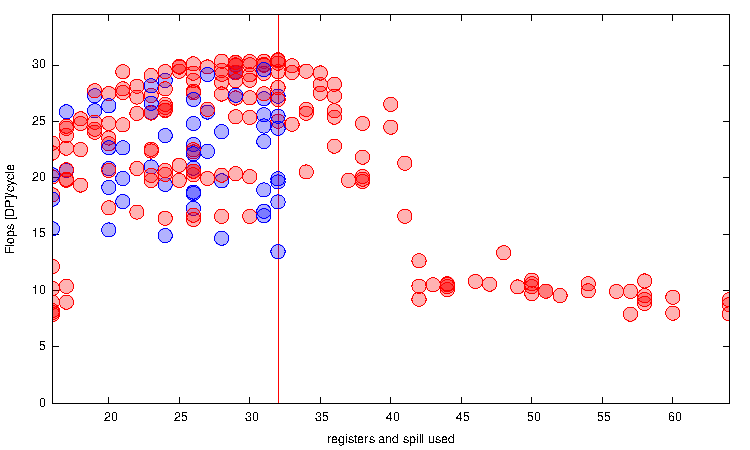
\includegraphics[width=\textwidth]{../benches/gemm/cascadelake-64x256x64/icc-2021.2.0.pdf}
  \caption{icc 2021.2.0}
  \end{subfigure}
  \begin{subfigure}[h]{0.45\textwidth}  
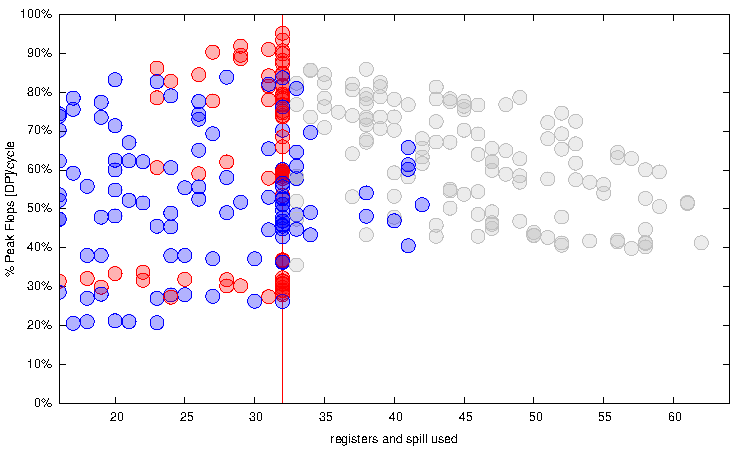
\includegraphics[width=\textwidth]{../benches/gemm/cascadelake-64x256x64/icc-19.1.3.pdf}
  \caption{icc 19.1.3}
  \end{subfigure}
  \begin{subfigure}[h]{0.45\textwidth}  
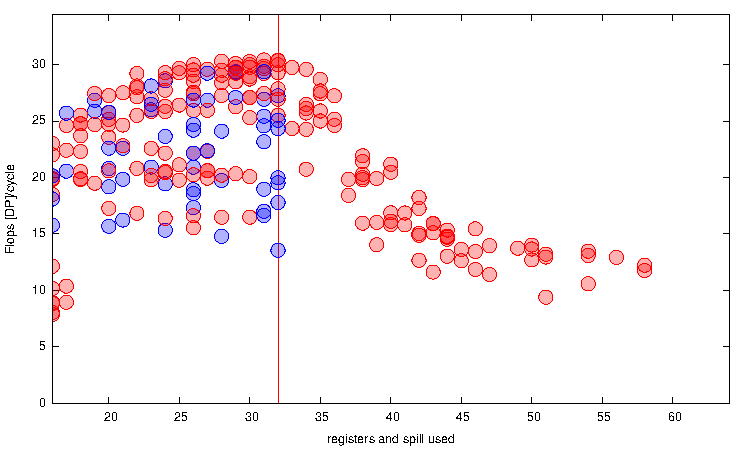
\includegraphics[width=\textwidth]{../benches/gemm/cascadelake-64x256x64/pbqp.pdf}
  \caption{Clang 15 with PBQP register allocation}
  \end{subfigure}
  \begin{subfigure}[h]{0.45\textwidth}  
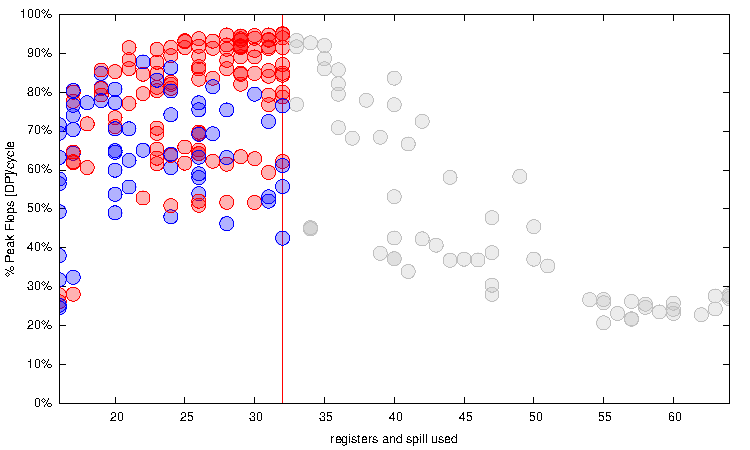
\includegraphics[width=\textwidth]{../benches/gemm/cascadelake-64x256x64/greedy.pdf}
  \caption{Clang 15 with Greedy register allocation}
  \end{subfigure}
  \begin{subfigure}[h]{0.45\textwidth}  
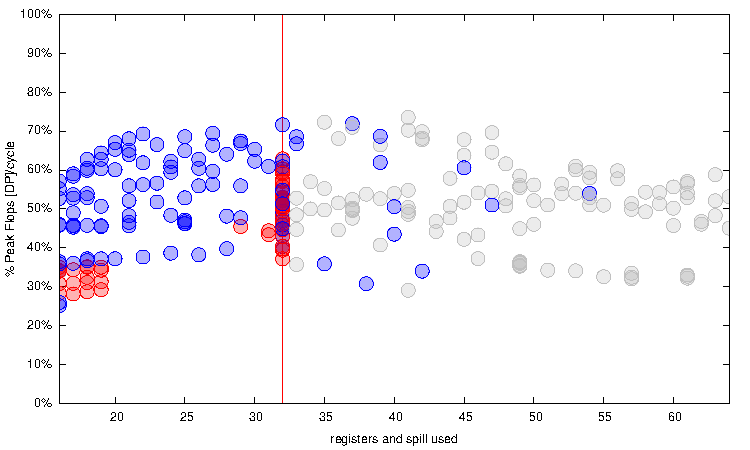
\includegraphics[width=\textwidth]{../benches/gemm/cascadelake-64x256x64/gcc-11.9.pdf}
  \caption{GCC 11.9}
  \end{subfigure}\hfill ~
  \caption{Block DGEMM Performance used on Intel CascadeLake with different compilers. The block (BI,BK,BJ) is 64x256x64. Each code represent a different register block size, obtained through the three unrolling factors. Codes with register block size $\leq 32$ are in blue (fit in register whatever the schedule), others in red.  \label{fig:cascadelake}}
\end{figure*}
 For all plots in Fig.\ref{fig:cascadelake}, the same codes with the same vectorization expressed with MIPP are
compiled. Points shown in blue correspond to codes that should not require
more SIMD registers than the physical registers (32 here, shown by the vertical red line), whatever
the scheduling chosen by the compiler. This is not the case for codes
shown in red, some schedules may manage to use only registers while
others will require spill code. The graphs show performance and the
cumulated register count required by the code, included the space on
the stack used by the spill. For instance, a value of 40 registers and
spill used indicates that the compiler was able to use all 32
registers and 8 additional spaces on the stack. With the exception of
GCC, other compilers manage to allocate less than 32 registers for all
blue codes. The max performance on this machine is normally 32 flops/cycles (with 2 FMAs operating on AVX512 vectors).  

There is no significant difference between icc version 2021 and Clang 15, either greedy or PBQP register allocations. This is expected since icc now is based on LLVM. GCC however fails significanlty, reaching  only 24 flop/cycle while other compilers reach 30-31 flop/cycle. 

The best codes for icc 2021 are: 8x2x3 (32/46), 8x1x3 (30/35), 7x3x3 (32/51), 7x2x3 (28/41), 6x4x3 (32/54), 6x3x4 (29/54), 6x3x3

\begin{figure*}[ht]
  \begin{subfigure}[h]{0.45\textwidth}
  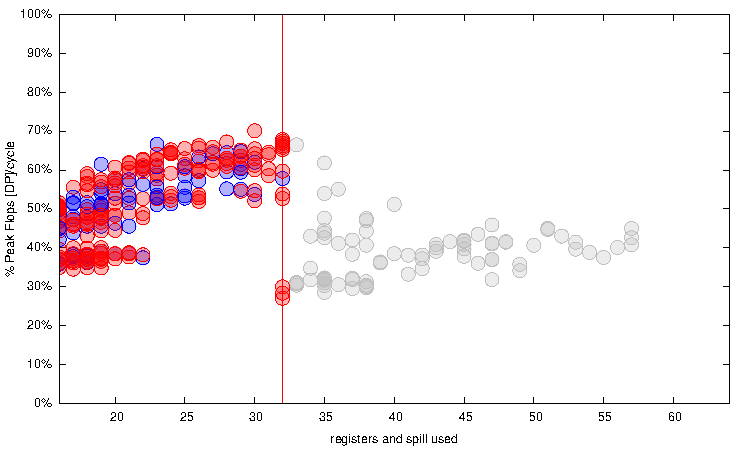
\includegraphics[width=\textwidth]{../benches/gemm/arm-64x256x64/greedy.pdf}
  \caption{clang 15}
  \end{subfigure}
  \begin{subfigure}[h]{0.45\textwidth}  
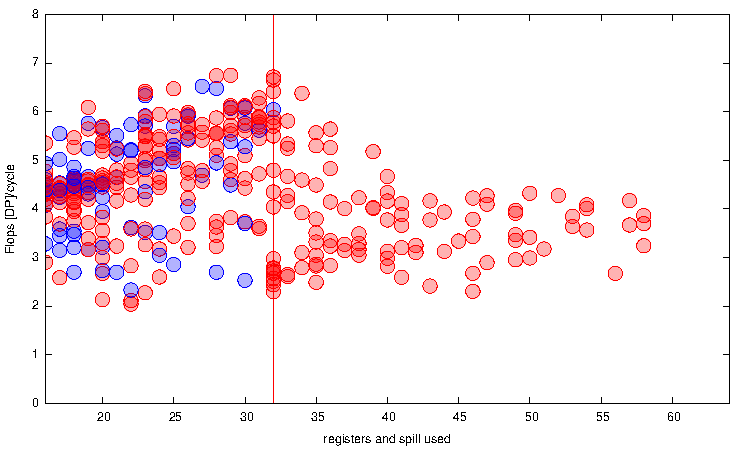
\includegraphics[width=\textwidth]{../benches/gemm/arm-64x256x64/openmp.pdf}
  \caption{clang 15 with OpenMP, SMT of 4}
  \end{subfigure}
  \begin{subfigure}[h]{0.45\textwidth}  
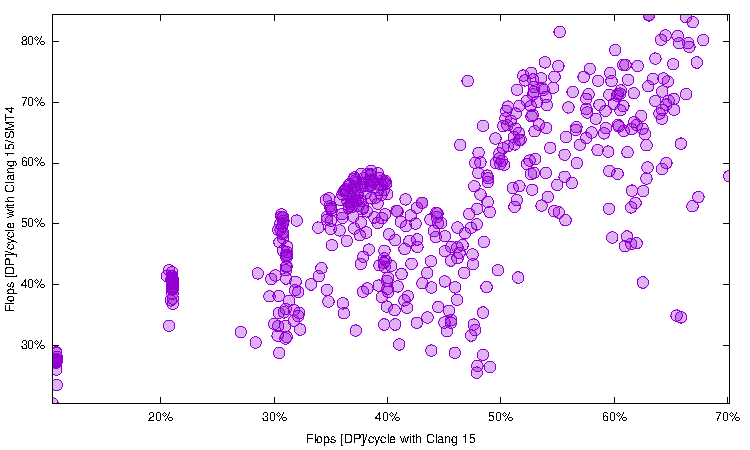
\includegraphics[width=\textwidth]{../benches/gemm/arm-64x256x64/clangxsmt.pdf}
  \caption{Correlation between Clang 15 without and with SMT4}
  \end{subfigure}
  \caption{Block DGEMM Performance used on Arm ThunderX2 with different compilers. The block (BI,BK,BJ) is 64x256x64. Each code represent a different register block size, obtained through the three unrolling factors. Codes with register block size $\leq 32$ are in blue (fit in register whatever the schedule), others in red. (c) show correlation between the two plots. \label{fig:cascadelake}}
\end{figure*}

\section{Related Works}
\section{Conclusion}
\label{sec:conclusion}

\bibliography{biblio}

\end{document}
